\chapter{Hardware Design}

The general hardware design was discussed in the previous chapter. This chapter
provides the detailed overview of the hardware design and implementation.


\section{Top Level Design}
The figure \ref{fig:hw:top} shows the top level design of the proposed hardware architecture.
The hardware consists of a set of pipelined MAC and divider units. The connection box
controls the inputs and outputs of each unit using the instruction bitstream fed 
through the input FIFO. The entire bitstream need not be stored on the FPGA and the 
available memory can be used only for data. The factors are stored in the BRAMs. Also the data from the matrix $A$ is
required only once, hence it can be streamed too. This will save the data loading
time of the matrix. 

\begin{figure}
    \centering
    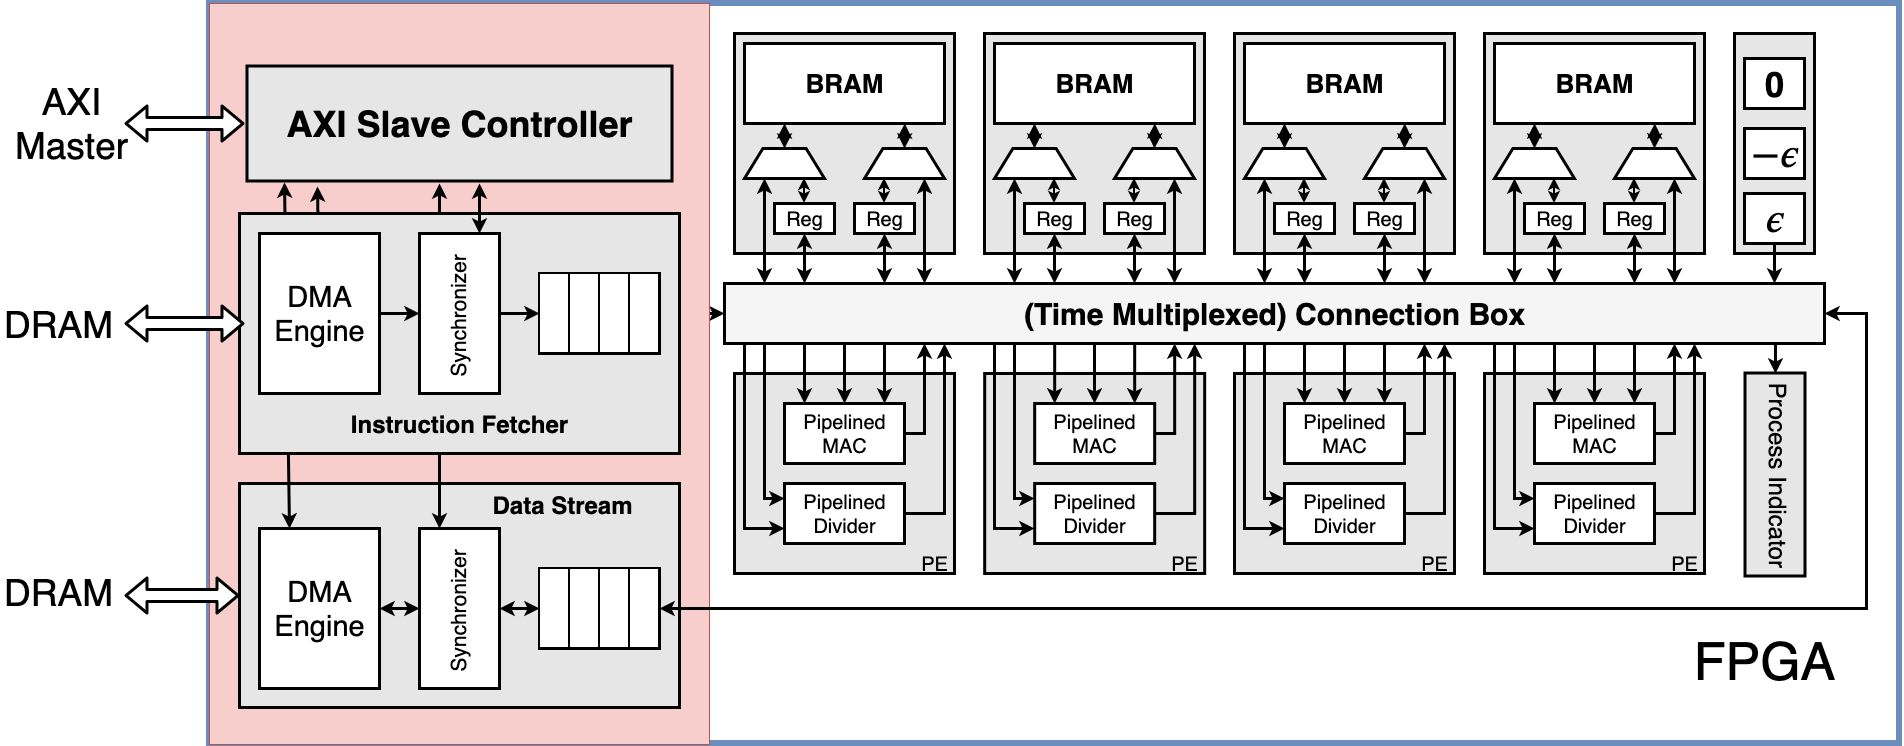
\includegraphics[width = \textwidth]{./Hardware/Hardware.jpg}
    \caption{Hardware architecure}
    \label{fig:hw:top}
\end{figure}


\section{Hardware Pivoting}

As discussed in earlier chapter, pivoting is very importing for the numerical
stability of the solution. But it is not feasible to regenerate the schedule 
for each matrix as the pivoting depends on the actual value. In order to ensure 
the numerical stability, we have to replace the tiny pivots 
$|a_{ii}| < \sqrt{\epsilon}||A|| = \epsilon_0$ with the $\sqrt{\epsilon}$, where $||A||$ is the norm 
of the matrix $A$. The $\epsilon$ is called as machine precision.
(e.g. $2^{-24}$ and $2^{-53}$ for single precision and double precision IEEE 754 formats).
This is acceptable in practical terms as the SPICE linear system solution is used as part of Newton-Raphson
iteration, and an occasional small error during the iterative process does not affect the integrity of the
final solution. \cite{machinePrecision}. Norm of the matrix can be calculated in the 
symbolic analysis step.

The pivoting block in the hardware is controlled by the instruction stream too. The result
of pivots are compared with the $\epsilon_0$ and will be replaced at the output of the PE. 
This block is only required at the outputs of the MAC units. To further simplify the design
we can ignore the comparison of mantissa. This allows us to use normal integer 
comparator to compare the magnitudes. This scheduler should generate an instruction bit suggesting 
the block to enable checking for the particular result.

\section{Bloack RAM Units}
Xilinix's Zynq 700 FPGA has true double port BRAMs, i.e. each BRAM can handle two 
read/write requests simultaneously provided there are is no write conflict in a single cycle.
These blocks can operate at much higher clock frequency (roughly 2X) than the Processing Elements. So we can use
time multiplexing the two available ports to emulate additional ports. Figure \ref{fig:hs:bram} shows
the structure of a single BRAM unit used in the implementation. Two available ports are generated with the help
of two clock with frequency ratio 2:1. These synchronous clocks are generated using the Xilinx's 
Clocking Wizard IP which uses on-chip PLLs.

\begin{figure}[H]
    \centering
    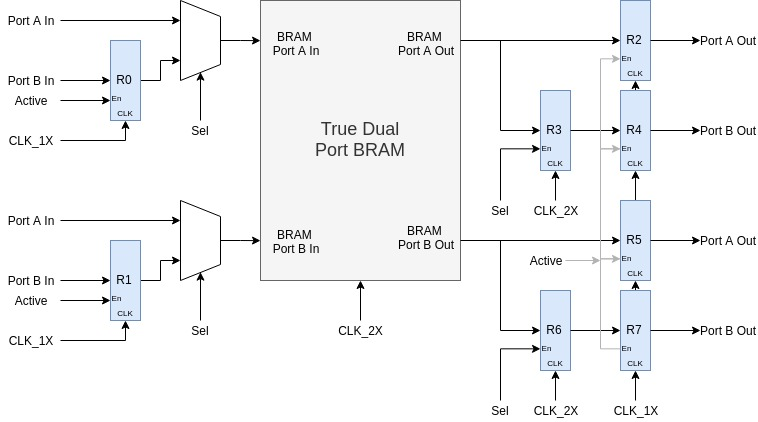
\includegraphics[width = 0.9\linewidth]{./Hardware/quadPortBRAM.jpg}
    \caption{BRAM unit with 4 time multiplexed ports}
    \label{fig:hs:bram}
\end{figure}


\begin{figure}
    \centering
    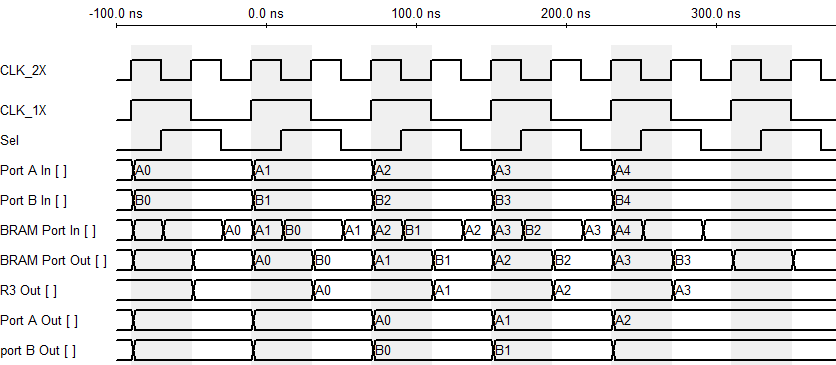
\includegraphics[width = 0.9\textwidth]{./Hardware/bramWave.png}
    \caption{Timing diagram for understanding the operation of Quad port BRAM}
    \label{fig:bram:wave}
\end{figure}

The operation od the quad port BRAM used in the project is shown in the figure \ref{fig:bram:wave}. Please 
note that the waveform is not time accurate and is just for explaining the operation process.
The Sel signal is generated by sampling the slow clock at the falling edge of fast clock. The figure 
\ref{fig:bram:sigGen} shows the generation of select signals and associated clocks along with reset and
active. The additional Active signal is generated to gate the clock signals for PEs to 
stall them when the next instruction is not available.

\begin{figure}
    \centering
    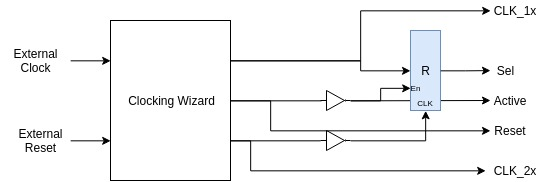
\includegraphics[width = 0.9\textwidth]{./Hardware/clock.jpg}
    \caption{Generation Clock and Select Signals}
    \label{fig:bram:sigGen}
\end{figure}

\section{Processing Elements}
All thge processing elements are pipelined to achieve higher throughput. Pipelining 
allows scheduler to assign independent operations in multiple clock cycles provided the operands
are available. The depth of pipeline for PEs is dependent on the operating frequency and 
the number of resources available on the target FPGA. In general lower latency PEs should
decrease the required number of clock cycles for the entire factorization process. But at the 
same time shallow pipelines have higher path delays and hence require slower clocks.

Xilinx provides readily available IPs for floating point operations. These IPs 
provide AXI Strem (AXIS) interface for both operands and result ports and can operate
in both blocking and non-blocking modes. For the scope of this project, the schedule
generated by the scheduler algorithm is cycle accurate and valid data is synchronized 
removing the need of blocking mode. This allows to reduce operation latency by reducing
pipeline depth and hardware resources.

\subsection{Multiply and Accumulate Unit}
The LU factorization process requires only a floating point multiply and subtract operations 
($Result = C - AB$). So we can remove the addition feature to save some of the resources.
The Xilinx's floating point IP supports operations of format $Result = AB \pm C $. this issue can
be easily resolved by inverting the sign bit of one of the multiplicands and using the multiply nad
add unit. The Xilinx's MAC units can utilize on-chip DSP Slices to achieve higher performance. 
\begin{equation*}
    \centering
    C - AB \rightarrow (-A.B) + C
\end{equation*}
For the scope of this project all the MAC units are set to utilize maximum number of DSP slices
since they are not being utilized in any other unit.

\pagebreak
\subsection{Divider Unit}
The Xilinx Floating Point Divider IP utilizes some variant of the radix-2 SRT division
algorithm and hence can not use DSP slices. This units are bulkier and hence have to be deeply
pipelined to operate. The speed grade of the target FPGA is one of the most dominating
factor in determining th depth of pipeline.

\section{Connection Box}
The connection box should allow connection from any output port to any input 
port for all the BRAMs and PEs. This can be achieved with multiplexers. All
the ports of both BRAMs and PEs forms the set of input signals for these multiplexers.
The select signals are provided by the instruction register. The number of 
the multiplexers depend on the number or PEs, number of BRAMs and number of ports at 
each BRAM. This multiplexers can be pipelined to achieve desirable operating frequency.
This allows some scalability to the system. The additional latency can ber modeled 
as the delays of the PEs without affecting the scheduling algorithm. Since the 
location of all the elements is predetermined there is no need to transfer data from one 
BRAM t the other and hence we can eliminate connections from BRAM outputs to BRAM inputs.
